%%% describe all the experiments performed and their statistical analysis
\chapter{Results} % at least 10, maximum 40 pages

%%%%%%%%%%%%%%%%%%%%%%%%%%%%%%%%%%%%%%%%%%%%%%%%%%%%%%%%%%%%%%%%%%%%%%%%%%%%%%%%
\section{Characterization of Physicochemical Properties}
  \subsection{Stacking Potential}
    \subsubsection{Obtaining the Datasets}
      A total of $83500$ protein structure files were downloaded from the PDB, some of which also contained ligands. Similarly, $3032$ structures with protein and nucleic acid complexes where downloaded, with the presence of ligands in some of them. From these two datasets, $22786$ unique ligand IDs were observed. The CIF files for these ligands were also downloaded from the PDB.

    \subsubsection{Detecting Aromatic Groups in Ligands}
      The first method of detection (parsing the SMILES strings) found aromaticity in $18211$ ligands from the dataset, while the second method (simple topological examination of the structures) found aromatic groups in $19096$ ligand files. From these ligands, $388$ were detected only by the first method, while $1273$ were detected only by the second method, meaning that the detection methods disagreed in the case of $1661$ ligands (figure \ref{fig:results/stacking_detection}).

      \begin{figure}[H]
        \centering
        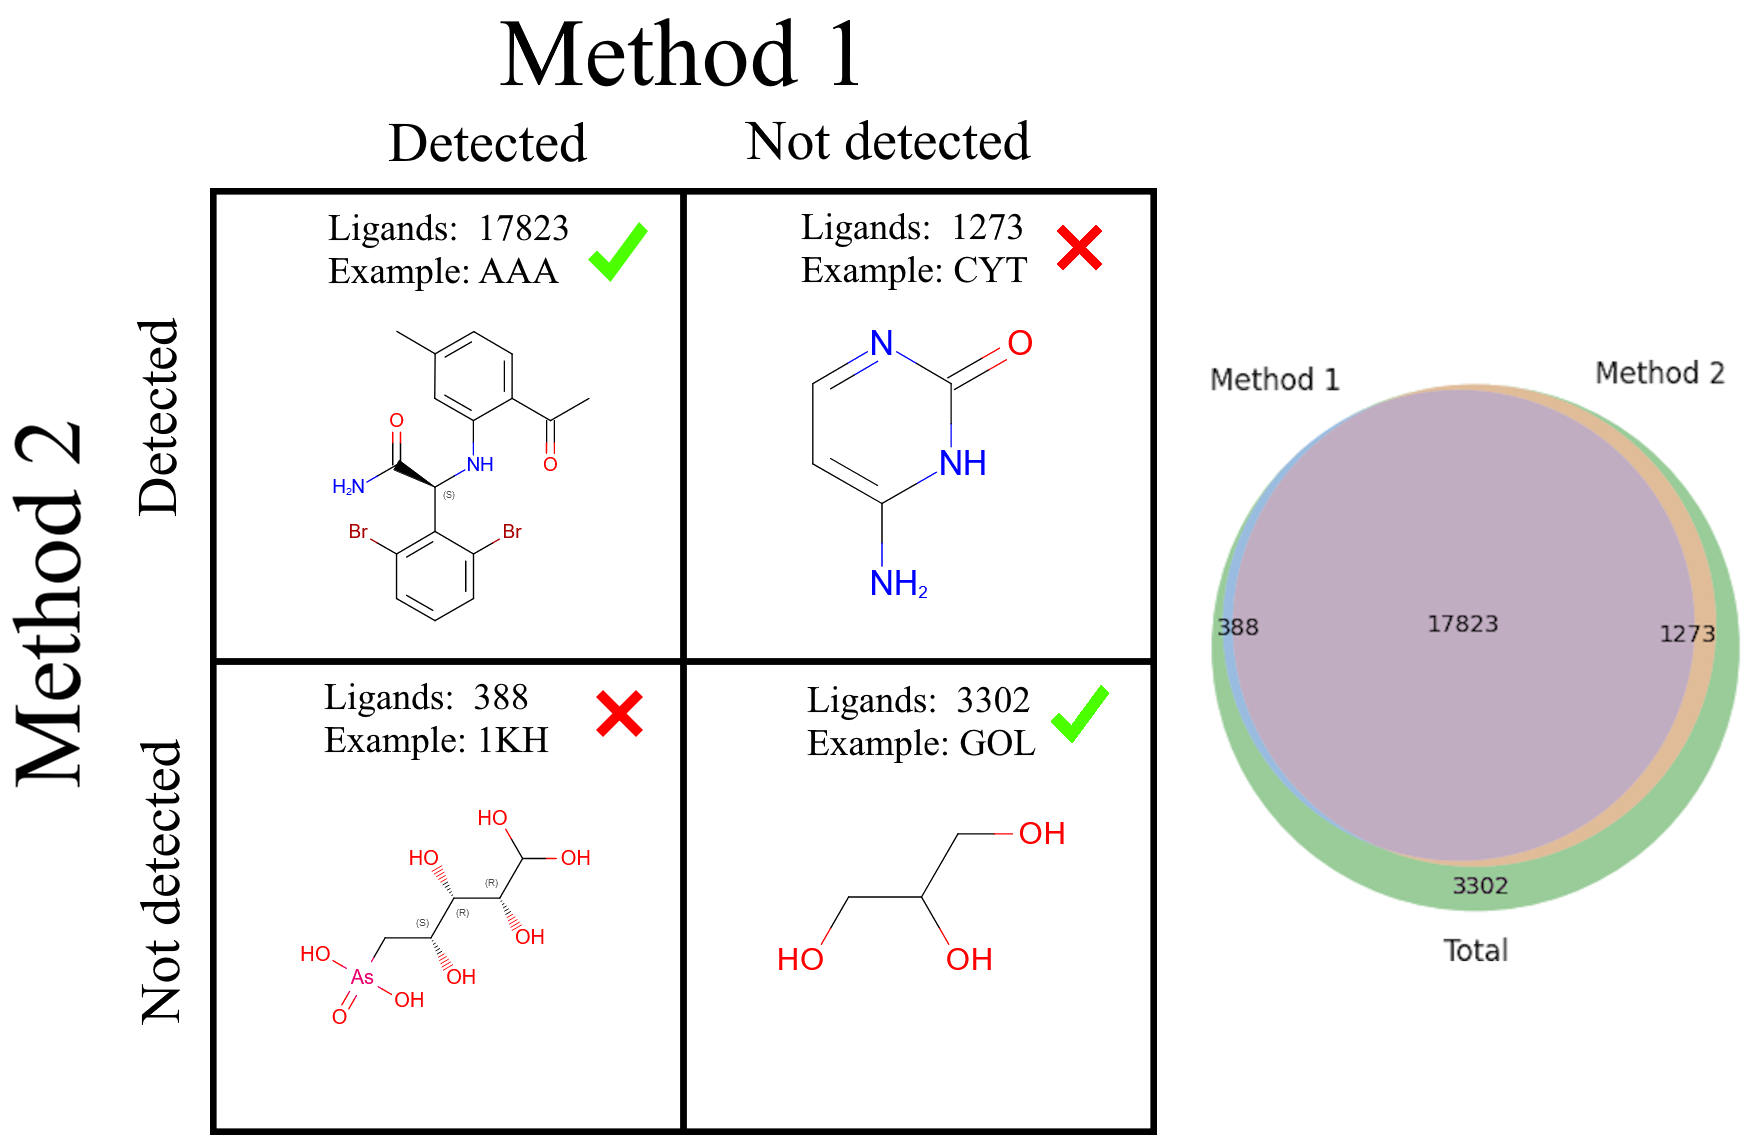
\includegraphics[width=0.8\textwidth]{figures/results/stacking_detection.png}
        \caption{\label{fig:results/stacking_detection} [TODO: description]}
      \end{figure}

      Some CIF files from the dataset had faulty SMILES strings (such as including the ligand name as a placeholder) or did not report correctly the aromaticity of the ligands. An example of the latter is the nucleic acid cytosine (CYT in figure \ref{fig:results/stacking_detection}), which is not properly identified as aromatic despite being a classic example of a very biologically relevant aromatic group. This also was observed in uracyl and other pyrimidines.

      The opposite situation also happened, where the SMILES string apparently contained aromatic atoms because lowercase symbols were found. However, this sometimes corresponded unrelated heavy atoms. An example of this occurance is the ligand 1KH in figure \ref{fig:results/stacking_detection}, whose arsenic atom is represented by "As" in the SMILES string, so the first method recognized the lowercase "s" as an aromatic sulfur. The second method however immediatly discarded the ligand as it is acyclic.

      Some other instances with complex combinations of aromatic and non-aromatic rings (oftentimes connected by one or two atoms) presented problems for the second method, while being correctly reported in the first method. For these reasons, these $1661$ were manually inspected to clarify whether aromaticity was present or not. At the end of this process, $18298$ ligands (accounting for $80.3 \% $ of the original dataset) were found to present a combined total of $34807$ aromatic groups (on average, 1.9 aromatic groups per ligand).

    \subsubsection{Sampling of Aromatic Interactions}
      A total of $4843590$ interactions were sampled from the PDB dataset. The interaction datapoints were grouped according to their $\alpha$ and $\beta$ values. The average interaction distance for each group and their abundance in the dataset were inspected by means of a histogram (figure \ref{fig:results/stacking_sampling}.a).

      However, many of these datapoints could correspond to non-interacting aromatic groups in close proximity, which most likely occurs in \textbf{aminoacid-aminoacid} pairs. By filtering these out, $696676$ interactions remain, which accounts to $14 \%$ of those originally observed. The histogram of these datapoints is significantly less noisy, where seemingly most of the points are condensed in some specific regions of the $(\alpha, \beta)$ space (figure \ref{fig:results/stacking_sampling}.b).

      \begin{figure}[H]
        \centering
        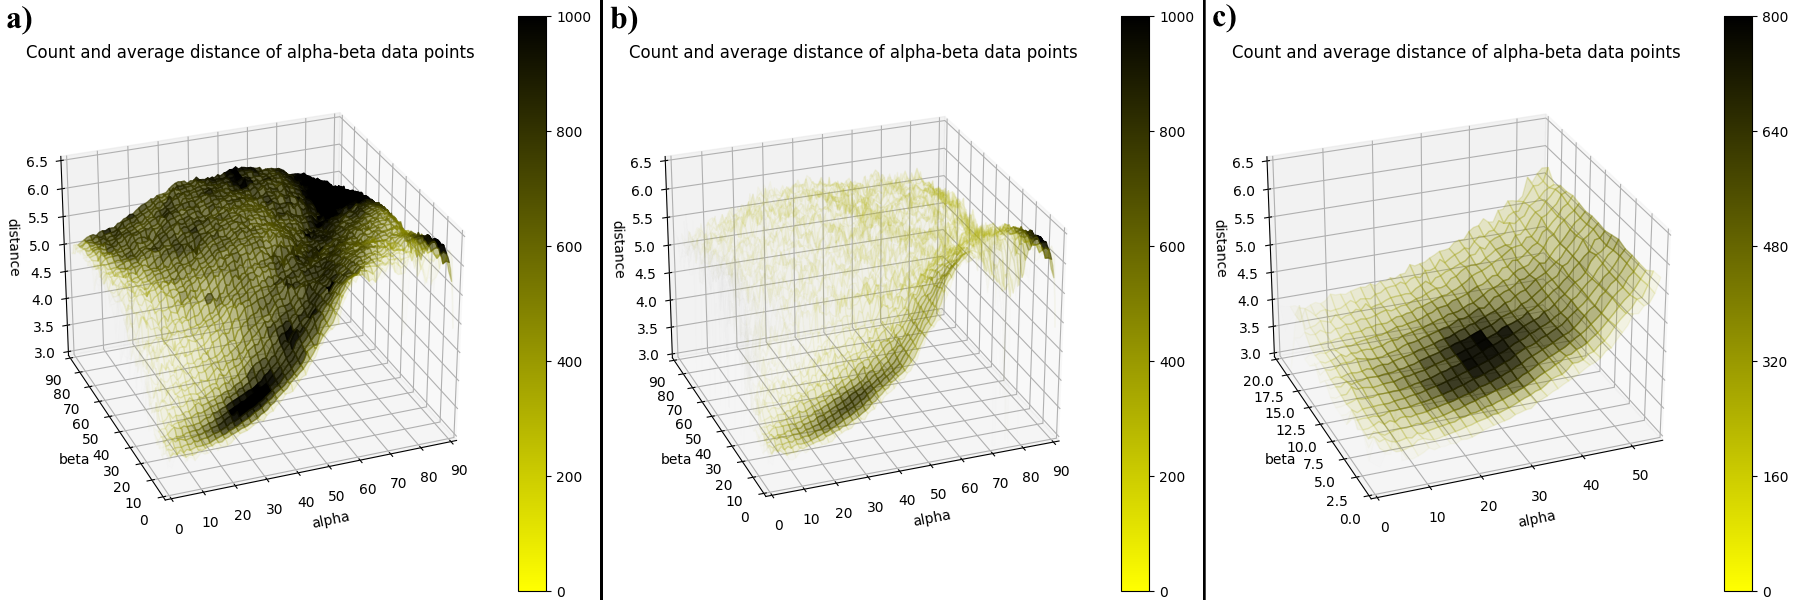
\includegraphics[width=1\textwidth]{figures/results/stacking_sampling.png}
        \caption{\label{fig:results/stacking_sampling} [TODO: description]}
      \end{figure}

      A high density of interaction datapoints can be observed at low $\beta$, high $\alpha$ values and relatively wide distances. This configuration mostly corresponds to base-pairing in PDB structures with nucleic acids, which can be further confirmed by filtering out \textbf{nucleic-nucleic} pairs (appendix figure \ref{fig:appendix/stacking_sampling}). Therefore, this region of points can be safely ignored.

      Another dense region of interaction datapoints can be observed spanning the range $\alpha \in [0,55], \beta \in [0,20]$. A total of $302651$ interactions are inside this range ($43 \%$ of the filtered datapoints). This range is also compatible with the theoretical configuration values of $\pi-\pi$ stacking potentials. Therefore, the empirical distribution of these values (figure \ref{fig:results/stacking_sampling}.c) will be used to define the model, suited to represent \textit{parallel-offset} stacking interactions specifically.

    \subsubsection{Model Definition}
      Some important observations must be noted before defining the stacking model:

      \begin{itemize}
        \item The histogram of the interactions of interest (figure \ref{fig:results/stacking_modeling}.a) reveals that varying the $\alpha$ value affects both the average distance of the points and their occurrence, while varying the $\beta$ value affects only the occurrence.
        \item The distance and the $\alpha$ value depend only on the position and normal vector of the aromatic group and the surrounding points in space, implying only three dimensions of space are needed.
        \item The $\beta$ value depends on the normal vector of both the actual aromatic group and the hypothetical aromatic group which interacts with it. This means that the $\beta$ value requires a \textit{$\beta$ angle} dimension, which raises the same issue found when theorizing the hydrogen bond potential model.
      \end{itemize}

      Therefore, even if it would be ideal to use all three parameters when building the model, the model was defined to assume an ideal beta value of either $\beta \approx 0^{\circ}$ (theoretically) or $\beta \approx 7.5^{\circ}$ (empirically, figure \ref{fig:results/stacking_modeling}.a). The datapoints were then grouped considering only their $\alpha$ and distance values and their occurrence observed in a histogram (figure \ref{fig:results/stacking_modeling}.b).

      \begin{figure}[H]
        \centering
        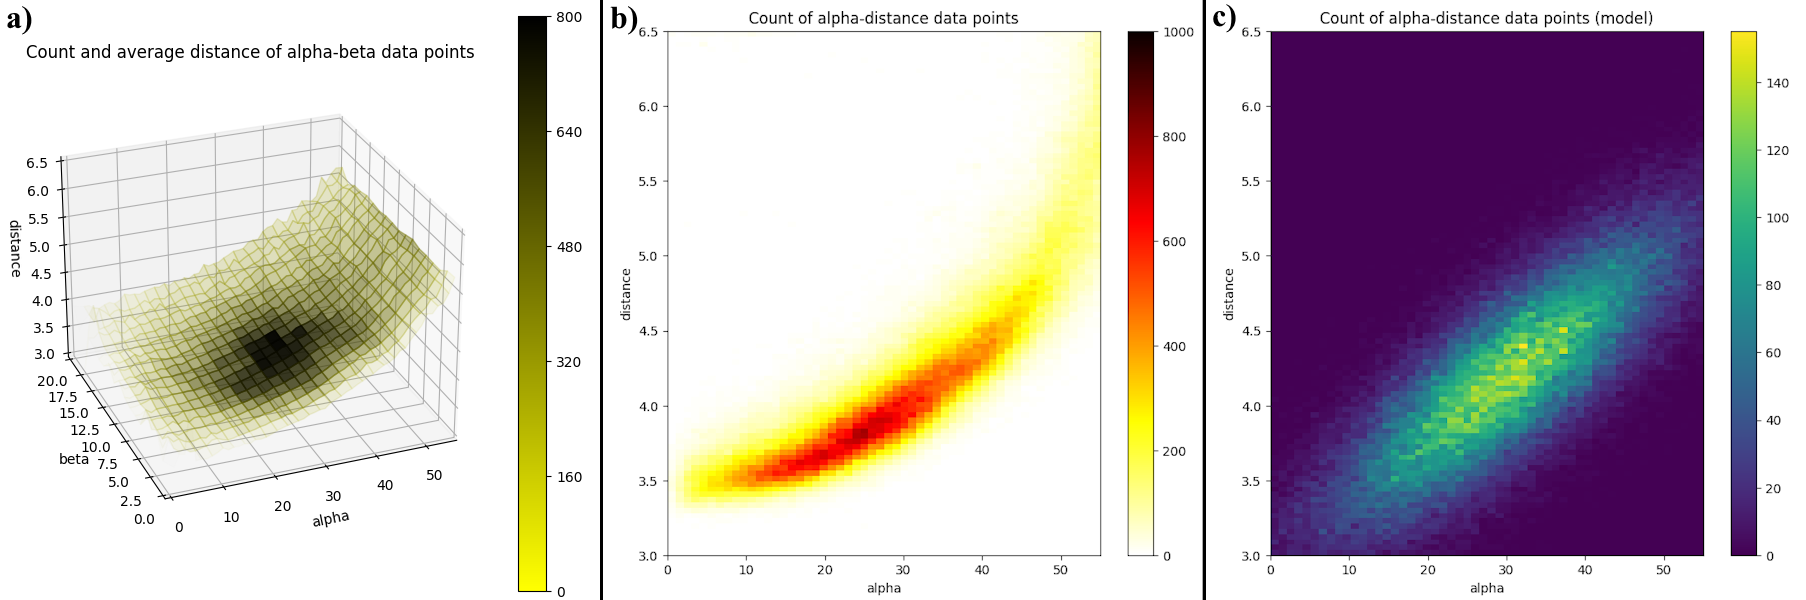
\includegraphics[width=1\textwidth]{figures/results/stacking_modeling.png}
        \caption{\label{fig:results/stacking_modeling} [TODO: description]}
      \end{figure}

      The empirical distribution resembles a skewed normal distribution. Given that the distortion is not extreme, an approximation was introduced and the model was empirically determined to have the shape of a \textbf{2D normal distribution}, with dimensions being distance and $\alpha$ angle (instead of just distance, which is the case of hydrogen bonds and hydrophobicity). Note however that the domain of the function still consists of three spatial dimensions, as $\alpha$ is only dependant on spatial coordinates and the \textit{normal vector} (which is not an input but rather a fixed parameter for each aromatic group) and it is calculated inside the function (analogous to how distance is calculated).

      The parameters were similarly obtained from the data histogram: $\mu = \begin{bmatrix} 29.98 \\ 4.19 \end{bmatrix}$ from the empirical average and $\sigma^2 = \begin{bmatrix} 169.99 & 6.62 \\ 6.62 & 0.37 \end{bmatrix}$ from the empirical covariance matrix. The shape of the modelled probability function can be observed in figure \ref{fig:results/stacking_modeling}.c.

      An isosurface representation of the output for a single aromatic group is presented in figure \ref{fig:results/visualize_stacking}.a. The stacking potential field of the aromatic group take the shape of two slightly flattened tori (i.e. "donut" shape), both below and above the aromatic plane. This shape is consequence of the spatial constraints imposed by the optimal distance and $\alpha$ values of the model ($\mu$) and the spread of the distribution ($\sigma^2$). According to this visualization, a stacking interaction will probably occur if an aromatic pharmacophorse is placed in any point of the volume covered by these tori.

      \begin{figure}[H]
        \centering
        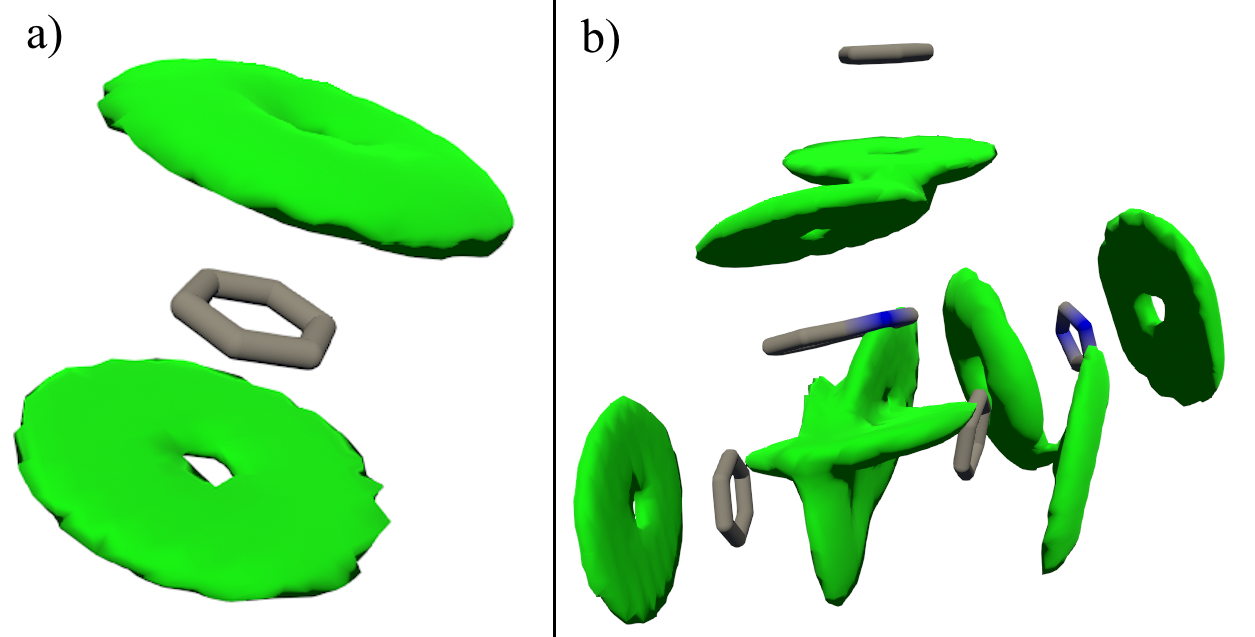
\includegraphics[width=0.7\textwidth]{figures/results/visualize_stacking.png}
        \caption{\label{fig:results/visualize_stacking} [TODO: description]. Trimming is turned off for clear visualization of the tori.}
      \end{figure}

      The model is a sum of the potential distribution defined by each aromatic group, which means that in actual pockets more than one pair of tori can be present. This will naturally overlap with each other in regions where multiple aromatic groups are in close vicinity (figure \ref{fig:results/visualize_stacking}.b). Points were multiple tori intersect imply a higher propensity for a pharmacophore to form one or multiple stacking interactions, potentially from both sides of the aromatic plane. The trimming step of the calculations will often cut out parts of the tori already occupied by the pocket atoms, so at the end the potential fields end up being mostly amorphous (figure [TODO: ref figure of some benchmark]).

  \subsection{Hydrogen Bonds Potential}
    [TODO: show the spheres formed by the univariate gaussian model]

    [TODO: description of the simultaneous positions where the ligand can have an ideal angle for the given distance]

  \subsection{Electrostatic Potential}
    [TODO: show the christmas tree effect and compare it to logAPBS]

    [TODO: show the log and trimmed log plots]


%%%%%%%%%%%%%%%%%%%%%%%%%%%%%%%%%%%%%%%%%%%%%%%%%%%%%%%%%%%%%%%%%%%%%%%%%%%%%%%%
\section{Development of Visualization Methods}
  \subsection{Graphical User Interface}
    % Pocket Sphere stuff
    [TODO: pocket sphere and changing its size vs pocket sphere off]

    [TODO: cartoon vs surface representation]


  \subsection{Potentials Visualization}
    % Representation of the potential grids in UnityMol
    [TODO: trimmed vs not trimmed sphere]

    [TODO: cloud vs isosurface]


%%%%%%%%%%%%%%%%%%%%%%%%%%%%%%%%%%%%%%%%%%%%%%%%%%%%%%%%%%%%%%%%%%%%%%%%%%%%%%%%
\section{Benchmarking}
  \subsection{Protein Systems}
    [TODO]

  \subsection{RNA Systems}
    [TODO]


%%%%%%%%%%%%%%%%%%%%%%%%%%%%%%%%%%%%%%%%%%%%%%%%%%%%%%%%%%%%%%%%%%%%%%%%%%%%%%%%
